\documentclass[10pt,twocolumn]{article}

% ---------- PACKAGES ----------
\usepackage[utf8]{inputenc}
\usepackage[T1]{fontenc}
\usepackage[british]{babel}
\usepackage{csquotes}
\usepackage{graphicx}
\usepackage{booktabs}
\usepackage{amsmath}
\usepackage{caption}
\usepackage{subcaption}
\usepackage{geometry}
\geometry{margin=1.8cm}
\usepackage{titlesec}
\usepackage{hyperref}
\usepackage{xcolor}
\usepackage{setspace}
\usepackage{tikz}
\usepackage{pgfplots}

\usepackage{lmodern}
\renewcommand{\familydefault}{\sfdefault} % sans-serif


\pgfplotsset{compat=1.18} % oder aktuelle Version
\usepackage[style=apa, backend=biber, sortcites=true, doi=false, isbn=false, url=true, giveninits=true]{biblatex}
\DeclareLanguageMapping{british}{british-apa}

\addbibresource{references.bib}

% ---------- TITLE & AUTHOR ----------
\title{\textbf{Form of Explanation: Explainability vs.\ Explicability of an Automation Aid under Multitasking Load}}
\author{
\begin{tabular}{c}
Lilian Obidike, Sheethal Mohan Prabhu and Andrea Thelen\\[2pt]
\small \texttt{Group Z --- Human-Centered Trustworthy AI (CS5076-KP12) --- Summer term 2026}
\end{tabular}
}
\date{}

% ---------- SECTION FORMATTING ----------
\titleformat{\section}{\large\bfseries}{\thesection.}{0.5em}{}
\titleformat{\subsection}{\normalsize\bfseries}{\thesubsection}{0.5em}{}
\titleformat{\subsubsection}{\normalsize\itshape}{\thesubsubsection}{0.5em}{}

% ---------- BEGIN DOCUMENT ----------
\begin{document}

\twocolumn[

\maketitle

% ---------- HIGHLIGHTED ABSTRACT ----------
\begin{center}
\begin{minipage}{0.95\textwidth}
\setstretch{1.0}

\textbf{Introduction:} Explanations of automated systems can make operators \textit{feel} informed without improving what they actually \textit{know} --- explainability without explicability. We test whether the linguistic form of an explanation alone, with the information content kept constant, produces this dissociation under multitasking load.
\textbf{Methods:} In a small within-subjects study, participants supervised several tasks at once in OpenMATB while a not fully reliable automation aid supported one of them. Every participant worked with three explanation forms that all contained the same information: a verbose form, a contrastive form, and a contrastive form with an added action cue. After each block we measured how informed the participants felt and how accurate their mental model of the aid actually was, together with miss detection and the performance on the non-aided tasks.
\textbf{Results:} The verbose form felt most transparent, but the contrastive forms led to more accurate mental models, better detection of automation misses, better performance on the non-aided tasks, and lower workload. Most participants would also choose the contrastive form with the action cue again.
\textbf{Discussion:} The feeling of being informed and the actual knowledge moved in opposite directions, although all forms contained the same facts.
\textbf{Conclusion:} The form alone can create a feeling of transparency without knowledge. Explanations in supervisory settings should therefore be designed for explicability and not only for explainability.
\vspace{0.5em}

\textbf{Keywords:} Transparency, Explainability, Explicability, Mental Model, Cognitive Load, OpenMATB
\end{minipage}
\end{center}

\vspace{1em}
]

% ---------- INTRODUCTION ----------
\section{Introduction}

In many domains humans do not operate a system directly anymore, but supervise an automation and have to step in when it fails. For this, the operator needs to understand what the system is doing. The usual approach is to make the system transparent and let it explain its behaviour. However, an explanation that is given is not automatically an explanation that is understood --- especially when the operator is busy with several tasks at the same time.

In this study we test whether the wording of an explanation alone, with the information content kept the same, changes how informed operators \textit{feel} and how much they actually \textit{know} about the automation. For this we ran a small experiment in a multitasking environment with three differently worded explanation forms. Section~2 gives the background and defines our terms, Section~3 the research questions and hypotheses, Section~4 the method, and Sections~5--7 the results, discussion, and conclusion.

% ---------- BACKGROUND ----------
\section{Background}

\subsection{Definitions of terms}
We distinguish three related but separate constructs that recur throughout the lecture and the literature.

\textit{Transparency} is the degree to which a system provides the operator with insight into its inner workings, intentions, and reasoning process. Frameworks such as the Situation Awareness-based Agent Transparency (SAT) model describe transparency in terms of \textit{levels} of information the agent communicates --- what it is doing, why, and what it predicts \parencite{Chen2014,Mercado2016}.

\textit{Explainability} is the system's act of producing an explanation of what it did and how. It is a property of the system's output.

\textit{Explicability} is whether that explanation is presented in a way that it is actually understood and processed by the operator. It is a property of the human--system interaction, not of the output alone. Two explanations can be equally explainable (containing the same facts) yet differ in explicability.

\subsection{Relation to the lecture}
The project is anchored in two lecture topics: the \textit{transparency} block, which asks what level of information an aid should communicate, and the \textit{explainability and explicability} block, whose criteria for good explanations --- among them \textit{contrastiveness} and \textit{actionability}, drawn from the social-science account of explanation \parencite{Miller2019} --- motivate our design. Crucially, we deliberately do \textit{not} manipulate selectivity: selecting fewer facts removes information, which existing research already covers. We hold content constant and isolate \textit{contrastiveness} (how the same facts are framed) and \textit{actionability} (an added operator cue).

\subsection{Prior empirical work}
Transparency studies in human--agent teaming show that giving operators more information about an agent's reasoning and uncertainty can improve trust calibration and decision quality \parencite{Mercado2016,Stowers2017}, but they vary the \textit{level} of information without separating content from \textit{presentation}. In parallel, XAI research finds that explanations frequently increase users' agreement and subjective sense of understanding without a matching increase in objective understanding or error detection \parencite{Bansal2021,WangYin2021} --- findings that come almost entirely from single-task settings with full attention on the explanation.

\subsection{Research gap}
Two gaps follow. First, it is not known whether linguistic form alone --- holding information content constant --- affects perceived transparency and the operator's mental model. Second, the explainability--explicability dissociation has not been demonstrated under \textit{multitasking load}, the very condition under which supervisory operators usually work. If a status-log-style explanation makes operators feel informed without enabling them to anticipate the system's next action, automation errors may be missed, with far-reaching consequences in aviation, medical monitoring, or driving aids.

% ---------- OWN FOCUS ----------
\section{Research Question and Hypotheses}

\textbf{Research questions.} Both ask whether the \textit{linguistic form} of the aid's explanation --- content constant, under multitasking load --- matters, targeting the two sides of the dissociation:

\begin{description}
  \item[RQ1 (subjective).] Does the form of the explanation change the operator's \textit{subjective transparency} --- the feeling of being informed? \textit{(addressed by H1)}
  \item[RQ2 (objective).] Does the form of the explanation change whether the operator's \textit{mental model actually updates} --- objective explicability? \textit{(addressed by H2)}
\end{description}

We compare three forms of explanation that all communicate the same facts (Section~\ref{sec:forms}); the comparison is between \textit{linguistic forms}, not amounts of information. H1 and H2 are the load-bearing pair --- that they predict opposite directions is the signature of the dissociation; H3 and H4 are supporting hypotheses.

\begin{description}
  \item[H1 (verbose feels more transparent).] Subjective transparency is highest under the verbose form (F1), even though the information content is identical across forms.
  \item[H2 (contrastive form improves explicability).] Post-block mental-model accuracy is highest under the contrastive forms (F2/F3), even though the information content is identical across forms.
  \item[H3 (contrastive form improves miss detection).] Because the action-relevant fact is easier to read off a contrastive panel, participants detect a higher proportion of automation-missed events under F2/F3 than under F1.
  \item[H4 (saved reading time is redeployed).] Participants achieve higher performance on the non-aided tasks (communications and resource management) under F2/F3 than under F1.
\end{description}

H1 reflects that a detailed stream of information makes the system \textit{feel} maximally informative; H2--H4 follow from the prediction that contrastive framing and an actionable cue make the same information easier to process under load, freeing attention for the events that matter.

% ---------- REFERENCE TO OHTER GROUPS ----------
\subsection{Reference to other groups}
Most groups built on the lecture constructs: transparency, trust, mental models, workload. The closest to us vary the \textit{wording} of the aid's messages: \textbf{AH~Group} (actionable vs.\ generic), \textbf{Group~P} (concrete vs.\ vague warnings), \textbf{Group~A} (calm vs.\ neutral tone), team \textbf{It-takes-two} (reason-giving vs.\ status-only), and especially \textbf{Group~K}, which compares no/vague/clear failure messages with length matching. Other groups are more distant: they add an explanation rather than reframing it, manipulate the system itself (reliability, automation level, task load), or treat trust as a personal trait or social signal.

Unique to us is that we hold the \textit{information content constant} across all three forms, isolating linguistic form rather than ``more vs.\ less'' explanation, and that we separate \textit{explainability} from \textit{explicability}, predicting opposite directions (H1 vs.\ H2). Where most colleagues ask ``does clearer explanation raise trust?'', we ask whether an explanation can raise the \textit{feeling} of being informed without improving what the operator actually \textit{knows} --- captured by an objective mental-model probe that, across all groups, only we use.

% ---------- METHOD ----------
\section{Method}

\subsection{Participants}
Twelve volunteers from our personal environment (family, friends, fellow students) took part, a convenience sample as suggested in the course. Six identified as female, six as male; the age ranged from 18 to 51 years ($M = 33.8$, $SD = 10.3$). Because OpenMATB resembles a video game, we also asked for gaming experience (3 a lot, 5 some, 4 none). Participation was voluntary and unpaid, and the data were stored under pseudonymous codes. All 12 participants completed all three blocks, which gives 36 analysable blocks without dropouts or exclusions.

\subsection{Materials}
The study runs on \textbf{OpenMATB} \parencite{Cegarra2020}, an open-source reimplementation of NASA's Multi-Attribute Task Battery \parencite{Comstock1992}. Participants perform three subtasks concurrently: \textit{system monitoring} (responding to out-of-range gauges and warning lights), \textit{communications}, and \textit{resource management} (pumps and tanks). Only system monitoring is supported by an automation aid; the other two compete for attention and are never aided.

The aid operates at approximately 78\% reliability. Each block contains \textbf{nine events}, one every 30\,s: five \textit{routine} events the aid handles in time, two \textit{near-misses} it handles just in time, and two \textit{misses} on which it does not act, so that --- if the information is perceived and processed --- the operator can still handle the event manually (7 of 9 $\approx$ 78\%). Behaviour, reliability, and failure timeline are identical across conditions; only the \textit{linguistic form} of the explanation panel changes.

\subsubsection{The three forms of explanation}
\label{sec:forms}
A panel fires on \textit{every} event in \textit{every} form (nine times per block), reporting the same facts: which indicator, in or out of range, whether the aid acted, and (for near-misses) the time-to-failure. The forms differ only in wording (Table~\ref{tab:forms}); the verbose form adds grammatical scaffolding and redundant exact sensor values but no new content with respect to catching a failure. This content matching is the core of the design: the F1$\leftrightarrow$F2 contrast isolates \textit{contrastiveness}, the F2$\leftrightarrow$F3 contrast \textit{actionability}.

\begin{table}[htbp]
\centering
\caption{The three forms of explanation, illustrated on a \textit{miss} (the aid did not act, so the operator must intervene). All forms report the same action-relevant facts and fire on every event; F1 embeds the facts in a verbose routine stream, F2 reframes them contrastively, and F3 adds an explicit operator cue on misses only.}
\label{tab:forms}
\begin{tabular}{@{}p{0.07\columnwidth}p{0.82\columnwidth}@{}}
\toprule
 & Description and example panel text \\ \midrule
F1 & \textit{Verbose.} Full-sentence status report on every cycle with exact sensor values. E.g.\ ``Cycle 05 (auto-aid) --- Scale-1 was 48.0, above the upper bound of 45.0; the automation did not act on this gauge.'' \\[4pt]
F2 & \textit{Contrastive.} Same facts, tight and contrastive. E.g.\ ``Skipped scale-1 --- auto-aid did not act.'' \\[4pt]
F3 & \textit{Contrastive + actionable.} F2 plus an explicit operator cue on misses. E.g.\ ``Skipped scale-1 --- auto-aid did not act. \textit{Check it yourself.}'' \\ \bottomrule
\end{tabular}
\end{table}

\subsection{Design}
The study uses a within-subjects design: each participant completes all three forms (F1/F2/F3), each paired with one of three gauge sets (A, B, C) containing different gauges and lights, so the post-block memory probe cannot be answered from another block's content. Form order is counterbalanced across participants with a Latin square to mitigate learning and order effects; because blocks are crossed with forms, by design every form meets every gauge set.

\subsection{Procedure}
Each session lasts approximately 20 minutes: 3 minutes practice, three 5-minute experimental blocks (one per form), then debriefing. After each block, questionnaires follow a fixed order --- the objective mental-model probe \textit{first} (before reflection contaminates it), then subjective transparency, then the workload item \textit{last}. A final preference questionnaire ends the session.

\subsubsection{Briefing and debriefing}
To avoid a bias, we did not tell the participants the research question, the hypotheses, or that the wording would change between the blocks. In the briefing they were told that the study investigates how people work with an automation aid while handling several tasks at once. During the practice phase they were instructed on the three subtasks and informed that the aid supports only the system monitoring, that it is \textit{not perfectly reliable}, and that they stay responsible for all tasks. Voluntariness, the option to stop at any time, and the pseudonymous storage were explained at the start. In the debriefing, after the final preference questionnaire, we explained the true purpose --- all three panels contained the same facts in different wording --- and answered questions.

\subsection{Measures}
Each measure maps onto one hypothesis. The questionnaire items are OpenMATB \texttt{genericscales} sliders presented after each block in the fixed order; every slider starts at a neutral position. The two behavioural measures (H3, H4) are read from the continuous platform log.

\subsubsection{H1 --- Subjective transparency}
Three sliders capture the \textit{feeling} of being informed (anchors in brackets):
\begin{itemize}
  \item ``The system told me what it was doing.'' \textit{(strongly disagree--strongly agree)}
  \item ``It was hard to keep track of what the automation was doing.'' \textit{(strongly disagree--strongly agree, reverse-scored)}
  \item ``The amount of information the system gave me felt about right.'' \textit{(strongly disagree--strongly agree)}
\end{itemize}
We developed these items ourselves, which is normally not recommended, because the existing validated instruments do not measure our construct: trust scales such as \textcite{Jian2000} measure trust in a system, not the feeling of being informed by it, and SAT-based transparency questionnaires \parencite{Chen2014,Mercado2016} ask how much reasoning \textit{content} the agent communicates --- exactly what we hold constant. Our three items instead cover (i) SAT Level~1, the feeling of knowing what the agent is doing \parencite{Chen2014}; (ii) the subjective cost of following the aid under load (reverse-scored, which also works against acquiescent responding); and (iii) the perceived information sufficiency, the aspect that is most directly affected when the wording changes but the content does not.

\subsubsection{H2 --- Mental-model probe}
Three yes/no sliders measure whether the operator's mental model actually updated. Within each block the aid \textit{handles} one active gauge (acts on it, and both near-misses land there) and \textit{misses} the other (never acts on it); each item targets one gauge by its role, so every correct answer is fixed by what happened in \textit{this} block, not by a constant strategy learned once (anchors in brackets):
\begin{itemize}
  \item ``Did the automation act on [gauge] at any point during this block?'' \textit{(no--yes; correct answer Yes for the handled gauge)}
  \item ``Did the automation FAIL to act on [gauge] at some point, leaving you to handle it yourself?'' \textit{(no--yes; correct answer Yes for the missed gauge)}
  \item ``Was there a close call (near miss) on [gauge] during this block?'' \textit{(no--yes; correct answer Yes for the handled gauge, which carries both near-misses)}
\end{itemize}
The probed gauges and their roles are counterbalanced across blocks, so the correct-answer pattern (Yes/Yes/No in one block, No/No/Yes in the others) embeds no fixed response heuristic. The responses are scored offline against the block ground truth to create an objective explicability score.

\subsubsection{H3 --- Detection of automation misses}
From the platform log we count how many automation-missed events (two per block) the participant detects and handles manually, compared across forms as a proportion; for caught misses we compute the reaction time from the moment the aid's panel fires to the participant's click on the relevant gauge or light.

\subsubsection{H4 --- Non-aided task performance}
\label{sec:h4-measures}
H4 tests whether the attention freed by an easier-to-read panel is redeployed to the two never-aided tasks. Both are read from the continuous platform log; we report the two standard MATB readouts per task \parencite{Comstock1992,SantiagoEspada2011,Cegarra2020}.

\paragraph{Resource management.} Two depleting tanks must be held near a target of 2500 units. We report (i) the \textbf{root-mean-square deviation (RMSD)} of tank level from target, averaged over tanks (lower is better) --- the typical deviation the operator allowed to build up --- and (ii) the \textbf{proportion of time within tolerance} ($\pm 500$ units; higher is better), the share of the block spent in an acceptable state.

\paragraph{Communications.} The operator must tune the named radio to the requested frequency on own-call-sign requests while ignoring distractors. We report (i) \textbf{response accuracy}, the proportion of own-call-sign trials answered correctly (higher is better), and (ii) \textbf{response time on hits} (lower is better), the more sensitive marker of spare attentional capacity under load \parencite{Cegarra2020}.

\subsubsection{Workload check}
A single mental-effort slider after each block:
\begin{itemize}
  \item ``How mentally demanding or overwhelming did this block feel?'' \textit{(very low--very high)}
\end{itemize}
This check is necessary because our assumed mechanism says that the verbose form costs more processing capacity under multitasking load; if F1 did not feel more demanding, we could not attribute H2--H4 to freed attention. A single item is sufficient because workload is here only a manipulation check and not an outcome for a hypothesis: single-item mental-effort ratings are validated and sensitive to load differences \parencite{Paas1992}, and a full multi-dimensional instrument like the NASA-TLX after every block would make the questionnaire phase between the blocks much longer.

% ---------- RESULTS ----------
\section{Results}

\subsection{Data set and analysis approach}
All 36 blocks (12 participants $\times$ 3 forms) entered the analysis; every session log was checked automatically against the study design (briefing form vs.\ panel form, gauge set vs.\ the gauges that actually failed, realised order vs.\ the Latin-square row), and no session was flagged. The metrics were computed from the raw OpenMATB logs in Python~3.13 and the figures were made using jupyter notebooks and the matplotlib library. Because of $n = 12$ we report only descriptive statistics and per-participant paired comparisons and use no inferential tests, since we could not credibly check their assumptions with this sample size. There were no missing questionnaire data; the only structurally missing values are the detection reaction times in blocks where no miss was caught (7, 5, and 6 of 12 blocks under F1, F2, F3). Because the achieved sample filled the Latin-square rows unevenly, the forms met the gauge sets slightly unequally (e.g.\ F1 met set~C in 5 of 12 blocks); each form still occurs 12 times.

Table~\ref{tab:results} summarises all block-level measures by form; the text below adds the per-participant paired comparisons that group means cannot show.

\begin{table}[t]
\centering
\caption{Results by form: mean ($SD$) over the 12 blocks per form (detection RT only over blocks with a caught miss, $n = 5/7/6$) and debrief votes (counts of 12). Bold: best form per row.}
\label{tab:results}
\footnotesize
\setlength{\tabcolsep}{3.5pt}
\begin{tabular}{@{}lrrr@{}}
\toprule
Measure & F1 & F2 & F3 \\ \midrule
\multicolumn{4}{@{}l}{\textit{H1 --- subjective transparency (1--7, higher = feels informed)}}\\
Transparency score & \textbf{5.28} (1.22) & 4.73 (0.96) & 4.78 (1.46) \\ \addlinespace
\multicolumn{4}{@{}l}{\textit{H2 --- mental-model accuracy (0--1, higher = better)}}\\
Explicability composite & 0.56 (0.33) & 0.64 (0.33) & \textbf{0.72} (0.28) \\
\quad``aid acted'' item & 0.33 (0.49) & \textbf{0.75} (0.45) & 0.58 (0.52) \\
\quad``aid failed'' item & 0.67 (0.49) & 0.67 (0.49) & \textbf{0.83} (0.39) \\
\quad``close call'' item & 0.67 (0.49) & 0.50 (0.52) & \textbf{0.75} (0.45) \\ \addlinespace
\multicolumn{4}{@{}l}{\textit{H3 --- detection of automation misses}}\\
Detection rate (0--1) & 0.33 (0.44) & \textbf{0.50} (0.48) & 0.46 (0.50) \\
Detection RT [s] & 5.06 (1.72) & \textbf{4.31} (0.70) & 4.55 (1.59) \\ \addlinespace
\multicolumn{4}{@{}l}{\textit{H4 --- non-aided task performance}}\\
RMSD from target [units] & 768 (663) & \textbf{744} (669) & 769 (736) \\
Time in tolerance [\%] & 44.3 (35.5) & 46.6 (37.4) & \textbf{50.0} (39.4) \\
Comms accuracy (0--1) & 0.38 (0.32) & \textbf{0.55} (0.43) & 0.50 (0.39) \\
Comms RT on hits [s] & 9.30 (1.03) & \textbf{9.06} (1.22) & 9.12 (1.66) \\
Composite index [$z$] & $-0.30$ (0.61) & 0.02 (0.55) & \textbf{0.28} (0.64) \\ \addlinespace
\multicolumn{4}{@{}l}{\textit{Workload check (1--7, lower = less demanding)}}\\
Mental demand & 4.22 (1.67) & 4.21 (1.44) & \textbf{3.67} (1.17) \\ \addlinespace
\multicolumn{4}{@{}l}{\textit{Debrief votes (counts of 12)}}\\
Most informative & \textbf{6} & 0 & \textbf{6} \\
Most useful for deciding & 2 & 2 & \textbf{8} \\
Most trusted & 4 & 1 & \textbf{7} \\
Least distracting & 3 & 2 & \textbf{7} \\
Would choose again & 1 & 2 & \textbf{9} \\ \bottomrule
\end{tabular}
\end{table}

\subsection{H1 --- Subjective transparency}
The verbose form felt most transparent (Table~\ref{tab:results}): F1 averaged 5.28 vs.\ 4.73/4.78, and 7 of 12 participants rated F1 above the mean of their two contrastive blocks (Figure~\ref{fig:dissociation}, solid line).

\subsection{H2 --- Mental-model accuracy (explicability)}
The objective probe showed the opposite order: the explicability increased step by step towards the contrastive forms, and 7 of 12 participants scored higher under F2/F3 than under F1 (3 lower, 2 tied). The largest single gap was on the ``did the aid act?'' item (0.33 under F1 vs.\ 0.75 under F2); the ``did the aid fail to act?'' item was best under F3. Figure~\ref{fig:dissociation} shows H1 and H2 together: the form that felt most transparent produced the least accurate mental model.

\begin{figure}[t]
\centering
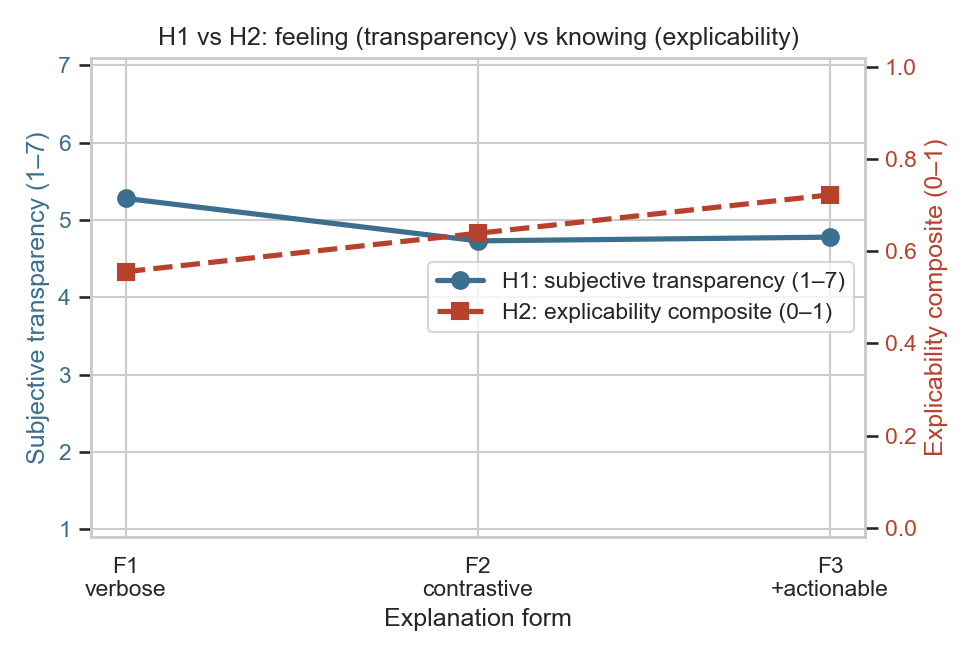
\includegraphics[width=0.85\columnwidth]{figures/h1_vs_h2_dissociation.png}
\caption{The dissociation ($n = 12$ per form): subjective transparency (H1, solid, left axis) peaks under verbose F1, while mental-model accuracy (H2, dashed, right axis) rises towards the contrastive forms --- opposite directions despite identical facts.}
\label{fig:dissociation}
\end{figure}

\subsection{H3 --- Detection of automation misses}
Detection of the two aid misses per block was lowest under F1 (rate 0.33 vs.\ 0.50/0.46); 5 of 12 participants detected more misses under the contrastive forms, 1 fewer, and 6 were tied --- 4 of them because they caught no miss in \textit{any} block. This floor effect is visible as the cluster at zero in Figure~\ref{fig:h3} and limits what H3 can show. On caught misses, participants also reacted fastest under F2 (Table~\ref{tab:results}).

\begin{figure}[t]
\centering
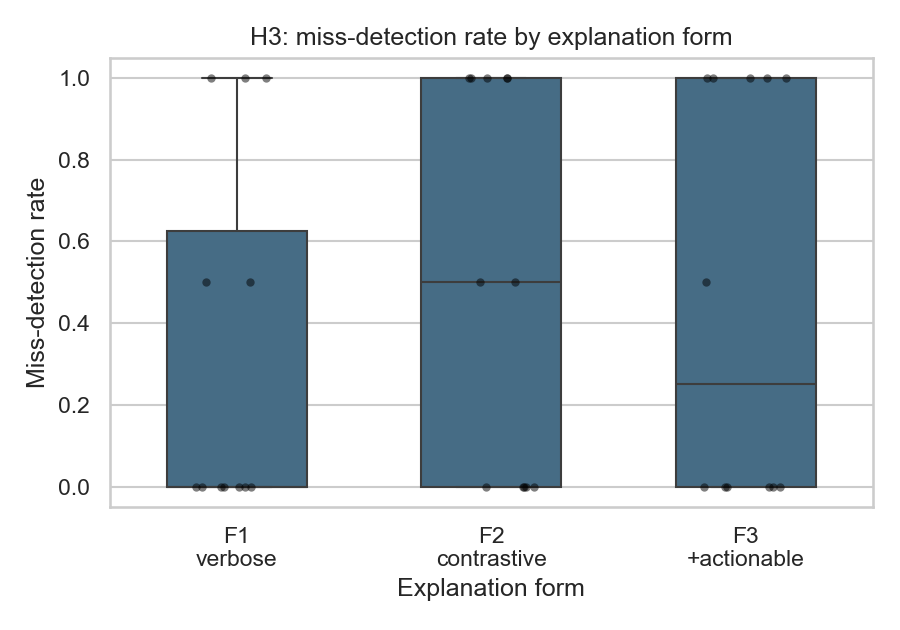
\includegraphics[width=0.85\columnwidth]{figures/h3_detection_rate_by_form.png}
\caption{H3: per-block miss-detection rates (two misses per block; boxes: quartiles, points: blocks). The distribution shifts up under F2/F3, but every form keeps a cluster at zero (floor effect).}
\label{fig:h3}
\end{figure}

\subsection{H4 --- Non-aided task performance}
In resource management the RMSD was almost identical between the forms (with a large spread between participants), but the time in tolerance increased with the contrastive forms; the communications accuracy and response time were also best there (Table~\ref{tab:results}). Summarising the four measures of Section~\ref{sec:h4-measures} in a composite index (each $z$-scored within participant, so every participant is their own baseline, sign-aligned so higher is better, then averaged), performance rose from $-0.30$ (F1) to $+0.28$ (F3), with 9 of 12 participants better under the contrastive forms (Figure~\ref{fig:h4}).

\begin{figure}[t]
\centering
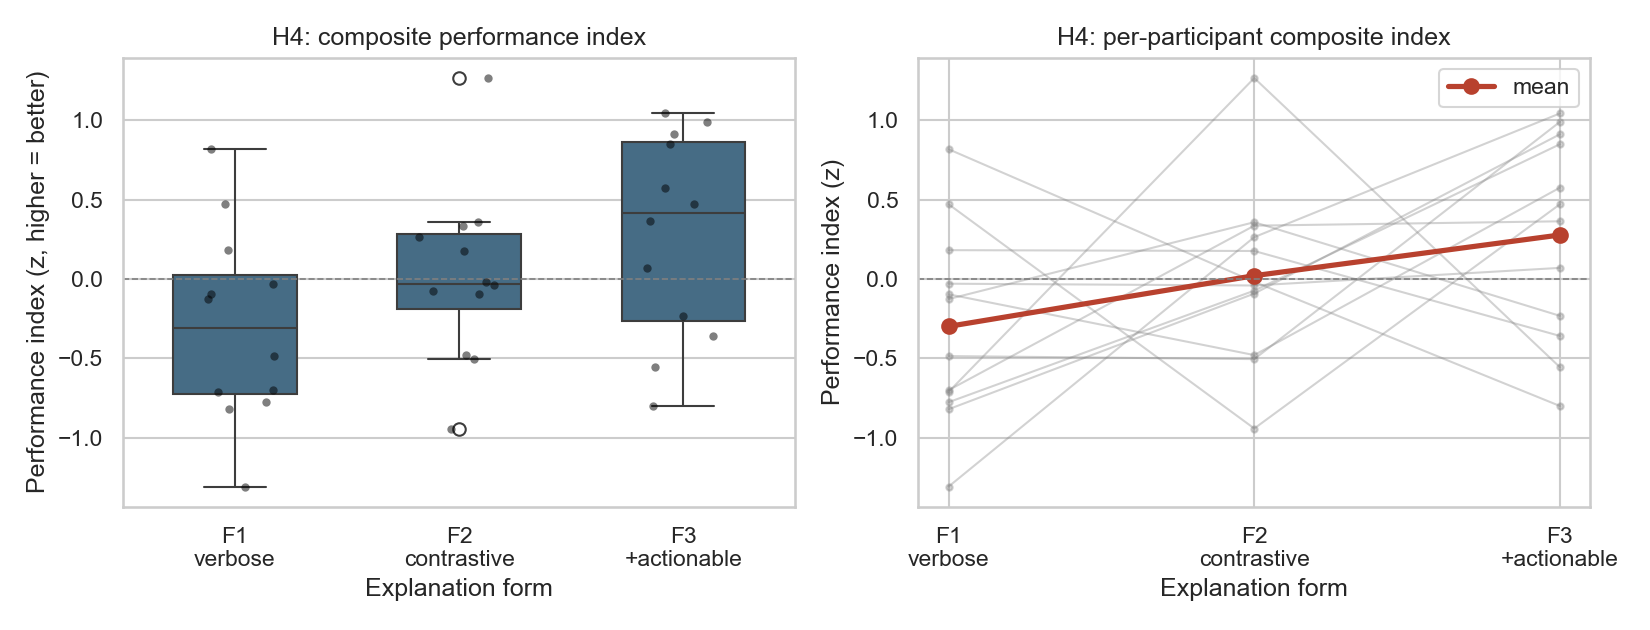
\includegraphics[width=\columnwidth]{figures/h4_composite_index_by_form.png}
\caption{H4: composite non-aided performance index (mean of the four sign-aligned $z$-scored measures; higher is better). Left: distribution per form. Right: per-participant lines, group mean in red, rising from $-0.30$ (F1) to $+0.28$ (F3).}
\label{fig:h4}
\end{figure}

\subsection{Workload check and preference debrief}
The reported mental demand was equal under F1 and F2 but clearly lowest under F3 (Table~\ref{tab:results}); 8 of 12 rated F1 above the mean of their contrastive blocks, which fits the assumed mechanism. In the final debrief (Figure~\ref{fig:pref}), F3 won four of the five questions --- most clearly ``would choose again'' (9 of 12) --- while ``most informative'' split evenly between F1 and F3 (6 votes each, none for F2). So the H1/H2 dissociation appears again inside a single questionnaire.

\begin{figure}[t]
\centering
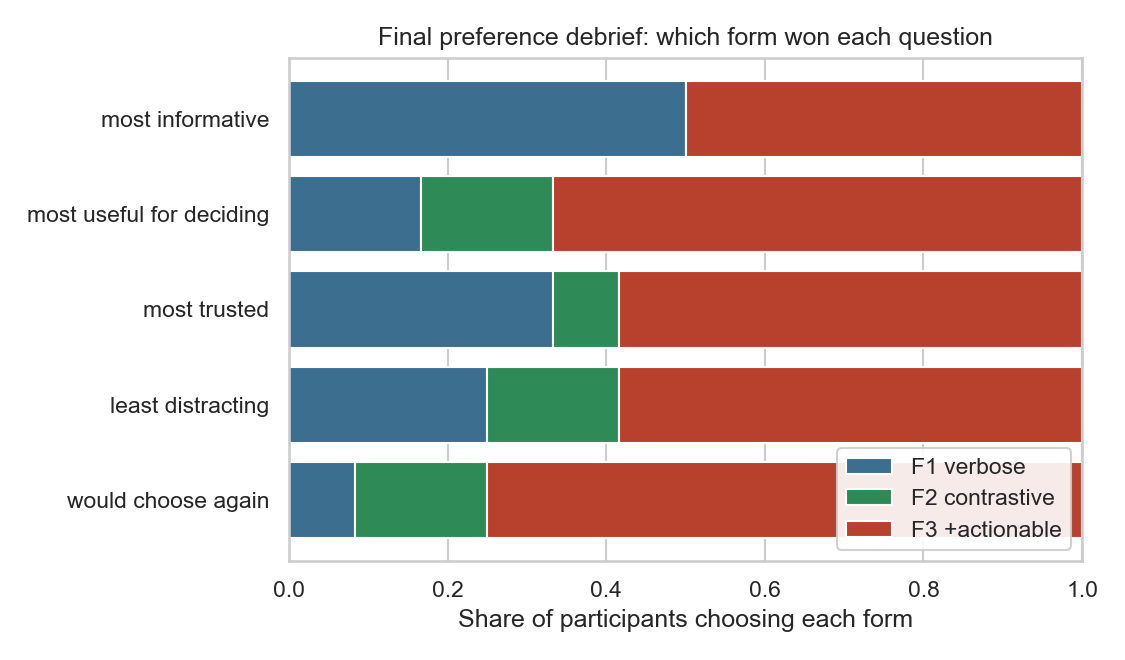
\includegraphics[width=0.92\columnwidth]{figures/preference_debrief_votes.png}
\caption{Debrief ($n = 12$): share of participants choosing each form per question (counts in Table~\ref{tab:results}). F3 dominates except ``most informative'', which splits evenly between F1 and F3.}
\label{fig:pref}
\end{figure}

% ---------- DISCUSSION ----------
\section{Discussion}

\subsection{Summary and interpretation}
Keeping the facts constant and changing only the wording moved our two key measures in opposite directions: the verbose form F1 felt most transparent (H1), but produced the least accurate mental model (H2), the lowest miss detection (H3), the worst non-aided performance (H4), and the joint-highest workload. Descriptively, all four hypotheses point in the predicted direction, and the central H1$\times$H2 dissociation shows as the crossover in Figure~\ref{fig:dissociation}. With $n = 12$ and without inferential statistics these patterns are only indications, not proof; with this caveat, both research questions get a careful ``yes'' --- the form alone changed the feeling of being informed (RQ1) \textit{and} the mental-model update (RQ2), and in opposite directions. This speaks to our research gap: the dissociation that was shown under full attention before \parencite{Bansal2021,WangYin2021} appears also under multitasking load; since the content was matched, it cannot come from some conditions containing more information. The result supports the view that contrastive framing makes the same facts usable \parencite{Miller2019} and complements the SAT-based transparency work \parencite{Chen2014,Mercado2016,Stowers2017}: at a fixed level of communicated information, the form still decides whether the information arrives.

\subsection{Unexpected findings}
Three results do not fit the simple picture. First, H1 was weaker than expected (7 of 12 in the predicted direction): the ``amount felt about right'' item may reward shortness as much as richness, which pulls some F2/F3 ratings up. Second, the ``did the aid act?'' probe item peaked under F2 and not F3 --- the F3 cue marks the \textit{misses}, so it plausibly sharpens the memory for misses (where F3 was best) rather than for routine actions. Third, a third of the sample never handled any missed event manually, in no single block. We read this as the multitasking load working as intended --- sometimes the panel is simply not processed at all --- but it leaves H3 only weakly supported.

\subsection{Critical reflection and limitations}
What went well: the content matching held (every panel fired on every event in every form), the automatic validation of each session protected us against mislabelled or misordered blocks (one aborted session was excluded and repeated), and the questionnaire data are complete for all 12 participants. The main limitations: (i) a small convenience sample and a descriptive analysis only --- the informative value is that of a pilot study, it can generate hypotheses but not test them; (ii) self-developed rating items, justified in Section~4.5 but not validated; (iii) only two automation misses per block, which makes the H3 scale coarse (0/0.5/1) and prone to floor effects; (iv) the forms met the gauge sets slightly unequally; (v) we measured the outcome of processing, not the processing itself --- without gaze data the ``freed attention'' mechanism stays an inference from the workload item. Next time we would recruit to a balanced square, include more miss events, and add eye tracking.

\subsection{Outlook}
Natural next steps are a replication with enough participants for inferential statistics, a factorial manipulation of the load to test whether the dissociation grows when attention shrinks (the central theoretical prediction), and a transfer test in a domain-specific simulator where a missed automation failure has realistic costs.

% ---------- CONCLUSION ----------
\section{Conclusion}
In a content-matched, within-subjects OpenMATB study ($n = 12$), the linguistic form of an automation aid's explanation separated feeling from knowing: the verbose form felt most transparent, while the contrastive forms led to more accurate mental models, better miss detection, better non-aided performance, and lower workload. For trustworthy AI the practical message is simple: a detailed explanation can create unjustified confidence, so explanations should be evaluated for \textit{explicability}, not only for explainability.

% ------------------------------------------------------------------------------------------
%
% Everything until here needs to be within the 6 pages.
% Only the acknowledgements and references are allowed to be on an additional page.
%
% ------------------------------------------------------------------------------------------

% ---------- ACKNOWLEDGEMENTS ----------
\section*{Acknowledgements}
We thank our twelve participants for volunteering their time, Nele Ru{\ss}winkel for the course framework and Rebecca von Engelhardt for the feedback on the study concept, and the authors of OpenMATB \parencite{Cegarra2020} for making the platform openly available.

% ---------- REFERENCES ----------
\printbibliography

\end{document}
